\section{Introduzione}

\subsection{Insiemi Numerici}
Un insieme di numeri è una raccolta di elementi. Alcuni degli insiemi che verranno utilizzati maggiormente in questo corso sono:
\begin{itemize}
    \item \textbf{N. Naturali} cioè tutti gli interi non negativi: $\mathbb{N}$ = $\{0, 1, 2, 3, 4, ...\}$.
    \item \textbf{N. Interi}: $\mathbb{Z} = \{..., -3, -2, -1, 0, 1, 2, 3, ...\}$.
    \item \textbf{N. Razionali}, cioè le frazioni: $\mathbb{Q} = \{\frac{p}{q}$ dove p e q $\in \mathbb{Z}$ e $q \neq 0\}$. \\
    Un sottoinsieme sono le \textbf{classi di equivalenza} che sono tutte le frazioni semplificate ai minimi termini. 
    \item \textbf{N. Reali}, che possono essere visti come tutti gli elementi rappresentabili su una retta: $\mathbb{R}$ 
\end{itemize}
\begin{note}
I vari insiemi si contengono fra di loro. ($\mathbb{N} \subset \mathbb{X} \subset \mathbb{Q} \subset \mathbb{R}$) 
\end{note}
\begin{note}
Esistono molti numeri reali che non sono razionali. Ess: $\sqrt{2}, \pi, ...$
\end{note}

\subsection{Intervalli}
\begin{definition}[Intervallo]
    $I \subseteq \mathbb{R}$ è un intervallo se $\forall \: x,\:y \in I$ tale che $x < y$. Allora ogni $z \in \mathbb{R}$ tale che $x < z < y$ sta esso stesso in I. [\ref{fig:intervallo}]
\end{definition}
\begin{wrapfigure}{l}{7cm}
    \vspace{-20pt}
    \centering
    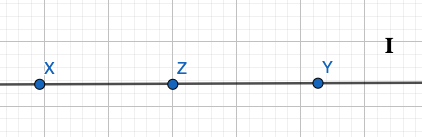
\includegraphics[width=5cm]{Intervallo.png}
    \caption{Tutto il segmento fra x e y deve stare in I}
    \label{fig:intervallo}
\end{wrapfigure}
\vspace{10pt}
I è un intervallo se ogni ogni volta che $x, y \in I$ e $x < y$, tutto il segmento tra x e y sta in I. Inoltre in I non ci sono "buchi" (discontinuità).
\\\\\\\\
\begin{example}
\vspace{-20pt}
Esempi di intervalli.\\ \\
Questo caso \textbf{è un intervallo} \hspace{3.2cm} Questo caso \textbf{non è un intervallo} fra A e D.
\begin{figure}[h!]
    \vspace{-10pt}
    \begin{subfigure}{.5\textwidth}
        \hspace{-50pt}
        \centering
        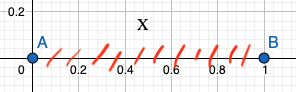
\includegraphics[width=6cm]{Esempio-intervallo-1.png}
        \caption{$A = \{x \in \mathbb{R} \: | \: 0<x<1\}$}
    \end{subfigure}
    \begin{subfigure}{.5\textwidth}
        \centering
        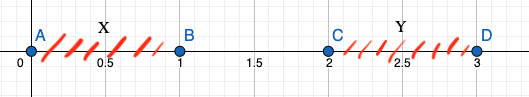
\includegraphics[width=7.5cm]{Esempio-intervallo-2.png}
        \caption{$C = \{x \in \mathbb{R} \: | \: 0<x<1 \: \: oppure\: \: z<x<3\}$}
    \end{subfigure}
\end{figure}
\end{example}

\newpage
\subsection{Notazione}
Con $a, b \in \mathbb{R}$ e con $a < b$ è possibile scrivere le notazioni in tabella \ref{tab:notazione-intervalli}.
\begin{table}[h!]
    \centering
    \setlength{\tabcolsep}{7pt}
    \renewcommand{\arraystretch}{2}
    \begin{tabular}{|c|c|c|} \hline
        [a, b] & Intervallo chiuso di estremi a e b & $\{x \in \mathbb{R} \: | \: a \leq x \leq b\}$ \\ \hline
        (a, b) & Intervallo aperto & $\{x \in \mathbb{R} \: | \: a < x < b\}$ \\ \hline
        [a, b) & Intervallo semi aperto a destra & $\{x \in \mathbb{R} \: | \: a \leq x < b\}$ \\ \hline
        (a, b] & Intervallo semi aperto a sinistra & $\{x \in \mathbb{R} \: | \: a < x \leq b\}$ \\ \hline
        [a, $+\infty$) & Semiretta chiusa a sinistra & $\{x \in \mathbb{R} \: | \: a \leq x\}$ \\ \hline
        ($-\infty$, b] & Intervallo semi aperto a destra & $\{x \in \mathbb{R} \: | \: x \leq b\}$ \\ \hline
        ($-\infty$, $+\infty$) & Insieme di tutti i numeri $\mathbb{R}$ & $\{x \in \mathbb{R}\}$ \\ \hline
    \end{tabular}
    \caption{Notazione Intervalli}
    \label{tab:notazione-intervalli}
\end{table}